
\section{TTS Move} % (fold)
\label{sec:tts_move}
    
    \begin{figure}[H]
        \centering
        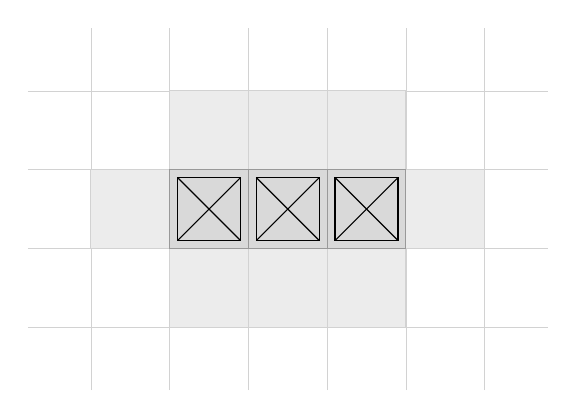
\begin{tikzpicture}
            \draw[step=1cm,gray!35!white,very thin] (.2,.2) grid (6.8,4.8);
            \foreach \x/\y in {2/1,3/1,4/1,1/2,2/3,3/3,4/3,5/2}
                \filldraw[fill=gray!15!white,draw=gray!35!white] (\x,\y) rectangle (\x+1,\y+1);
            \foreach \x/\y in {2/2,3/2,4/2}
            {
                \filldraw[fill=gray!30!white,draw=gray!80!white] (\x,\y) rectangle (\x+1,\y+1);
                \draw[black] (\x+.1,\y+.1) rectangle (\x+.9,\y+.9);
                \draw[black] (\x+.1,\y+.1) -- (\x+.9,\y+.9);
                \draw[black] (\x+.9,\y+.1) -- (\x+.1,\y+.9);
            }
        \end{tikzpicture}
        \caption{Horizontal Three--Tile Streak Selection}
    \end{figure}

    \begin{figure}[H]
        \centering
        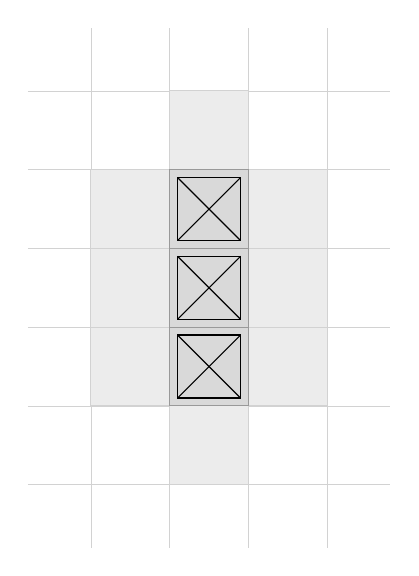
\begin{tikzpicture}
            \draw[step=1cm,gray!35!white,very thin] (.2,.2) grid (4.8,6.8);
            \foreach \x/\y in {2/1,1/2,3/2,1/3,3/3,1/4,3/4,2/5}
                \filldraw[fill=gray!15!white,draw=gray!35!white] (\x,\y) rectangle (\x+1,\y+1);
            \foreach \x/\y in {2/2,2/3,2/4}
            {
                \filldraw[fill=gray!30!white,draw=gray!80!white] (\x,\y) rectangle (\x+1,\y+1);
                \draw[black] (\x+.1,\y+.1) rectangle (\x+.9,\y+.9);
                \draw[black] (\x+.1,\y+.1) -- (\x+.9,\y+.9);
                \draw[black] (\x+.9,\y+.1) -- (\x+.1,\y+.9);
            }
        \end{tikzpicture}
        \caption{Vertical Three--Tile Streak Selection}
    \end{figure}

    \begin{figure}[H]
        \centering
        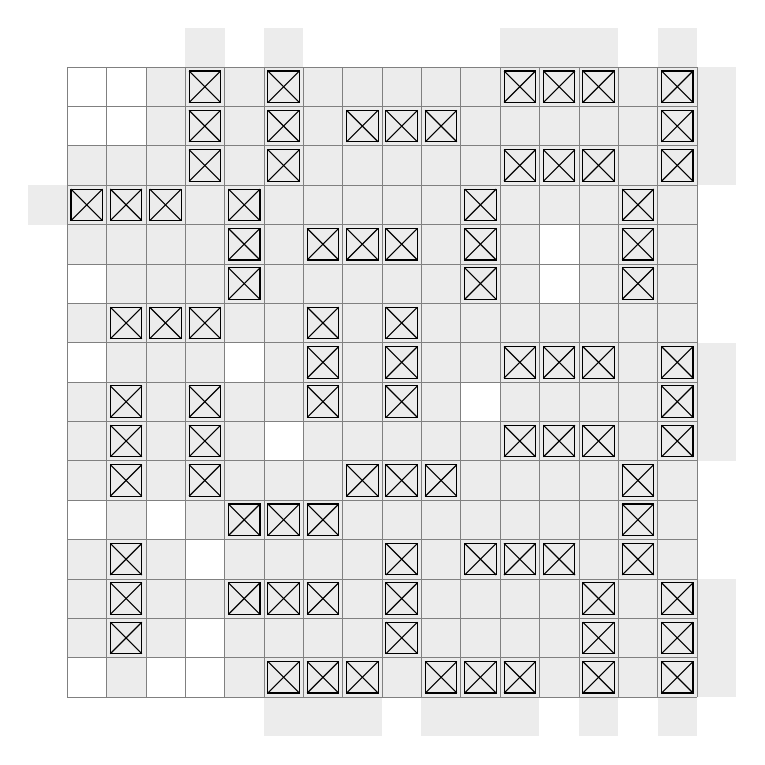
\begin{tikzpicture}
            %\foreach \x/\y in {2/1,1/2,3/2,1/3,3/3,1/4,3/4,2/5}
            %    \filldraw[fill=gray!15!white,draw=gray!35!white] (\x,\y) rectangle (\x+1,\y+1);
            \foreach \x/\y/\r in {.5/1/1,2.5/2/0,4/2.5/0,7/2/1,6.5/.5/1,0.5/3/1,0.5/6/0,3/0/0,2.5/1/0,4/1/1,5.5/1.5/0,5/0/0,7.5/.5/1,3/4/1,6/4/0,1.5/3/1,1/4.5/0,2/5.5/1,1.5/7/1,6/3/0,7.5/3.5/1,4/4/1,3.5/5.5/0,2.5/7/1,4/7/0,5/5.5/1,6/6.5/0,6/7.5/0,7.5/7/1,7/5.5/1}
            {
                \fill[fill=gray!15!white] (\x,\y) rectangle (\x+.5,\y+.5);
                \draw[black] (\x+.05,\y+.05) rectangle (\x+.45,\y+.45);
                \draw[black] (\x+.05,\y+.05) -- (\x+.45,\y+.45);
                \draw[black] (\x+.45,\y+.05) -- (\x+.05,\y+.45);

                \fill[fill=gray!15!white] (\x+.5*\r-.5,\y-.5*\r) rectangle (\x+.5*\r,\y-0.5*\r+.5);
                \draw[black] (\x+.5*\r-.5+.05,\y-.5*\r+.05) rectangle (\x+.5*\r-.05,\y-0.5*\r+.5-.05);
                \draw[black] (\x+.5*\r-.5+.05,\y-.5*\r+.05) -- (\x+.5*\r-.05,\y-0.5*\r+.5-.05);
                \draw[black] (\x+.5*\r-.5+.05,\y-0.5*\r+.5-.05) -- (\x+.5*\r-.05,\y-.5*\r+.05);

                \fill[fill=gray!15!white] (\x-.5*\r+.5,\y+.5*\r) rectangle (\x-.5*\r+.5+.5,\y+.5*\r+.5);
                \draw[black] (\x-.5*\r+.5+.05,\y+.5*\r+.05) rectangle (\x-.5*\r+.5+.5-.05,\y+.5*\r+.5-.05);
                \draw[black] (\x-.5*\r+.5+.05,\y+.5*\r+.05) -- (\x-.5*\r+.5+.5-.05,\y+.5*\r+.5-.05);
                \draw[black] (\x-.5*\r+.5+.5-.05,\y+.5*\r+.05) -- (\x-.5*\r+.5+.05,\y+.5*\r+.5-.05);

                \fill[fill=gray!15!white] (\x-.5*\r,\y+.5*\r-.5) rectangle (\x-.5*\r+.5,\y+.5*\r-.5+.5);
                \fill[fill=gray!15!white] (\x-.5*\r+.5*\r-.5,\y+.5*\r-.5*\r-.5) rectangle (\x+.5*\r-.5-.5*\r+.5,\y-.5*\r+.5*\r-.5+.5);
                \fill[fill=gray!15!white] (\x-.5*\r-.5*\r+.5,\y+.5*\r+.5*\r-.5) rectangle (\x-.5*\r+.5-.5*\r+.5,\y+.5*\r+.5*\r-.5+.5);
                \fill[fill=gray!15!white] (\x+.5*\r,\y-.5*\r+.5) rectangle (\x+.5*\r+.5,\y-.5*\r+.5+.5);
                \fill[fill=gray!15!white] (\x+.5*\r-.5+.5*\r,\y-.5*\r-.5*\r+.5) rectangle (\x+.5*\r-.5+.5*\r+.5,\y-.5*\r-.5*\r+.5+.5);
                \fill[fill=gray!15!white] (\x-.5*\r+.5+.5*\r,\y+.5*\r-.5*\r+.5) rectangle (\x-.5*\r+.5+.5*\r+.5,\y+.5*\r-.5*\r+.5+.5);
                \fill[fill=gray!15!white] (\x+\r-1,\y-\r) rectangle (\x+\r-1+.5,\y-\r+.5);
                \fill[fill=gray!15!white] (\x-\r+1,\y+\r) rectangle (\x-\r+1+.5,\y+\r+.5);
            }
            \draw[step=.5cm,gray,very thin] (0,0) grid (8,8);
        \end{tikzpicture}
        \caption{Example of feasible maximal selection of Three--Tile Streaks}
    \end{figure}

% section tts_move (end)